\documentclass[11pt,a4paper]{article}
\usepackage[margin=21mm,headheight=14pt]{geometry}
\usepackage{fontspec}
\setmainfont{lmroman10-regular.otf}[BoldFont=lmroman10-bold.otf,
ItalicFont=lmroman10-italic.otf,BoldItalicFont=lmroman10-bolditalic.otf]
\usepackage[english]{babel}
\usepackage{amsmath,amssymb,array,booktabs}
\usepackage{graphicx,float}
\floatstyle{ruled}
\newfloat{algorithm}{htbp}{loa}
\floatname{algorithm}{Algorithm}
\floatstyle{plain}
\usepackage{placeins}
\usepackage[numbers,sort&compress]{natbib}
\usepackage[unicode,colorlinks=true,citecolor=blue,urlcolor=blue,linkcolor=black]{hyperref}
\usepackage{fancyhdr}
\pagestyle{fancy}\fancyhf{}
\fancyhead[L]{\small TorusFlow}
\fancyfoot[C]{\small\thepage}
\renewcommand{\headrulewidth}{0.3pt}
\setlength{\parindent}{0pt}
\setlength{\parskip}{4pt}
\setlength{\emergencystretch}{3em}
\clubpenalty=10000
\widowpenalty=10000
\setlength{\abovedisplayskip}{5pt}
\setlength{\belowdisplayskip}{5pt}
\newcommand{\R}{\mathbb R}
\newcommand{\T}{\mathbb T}
\newcommand{\Z}{\mathbb Z}
\begin{document}
\thispagestyle{plain}
\begin{center}
{\Large\bfseries TorusFlow: Topological Phase Reconstruction\\[3pt]
from Spatiotemporal Data}
\end{center}

\section*{Problem statement}
Given synchronized sensor readings $Y=[y_0,\ldots,y_{N-1}]\in\R^{m\times N}$
sampled every $\Delta t$, recover their independent phases. Assume
\[
y_n=g(\theta_n)+\varepsilon_n,\qquad
\theta_{n+1}=\theta_n+\alpha\pmod{2\pi},\qquad
\theta_n\in\T^r=(\R/2\pi\Z)^r.
\]
The phase count $r$, smooth observation map $g:\T^r\to\R^m$ and phase
increment $\alpha\in\R^r$ are unknown; $\varepsilon_n\in\R^m$ is noise.
Assume $k^\top\alpha\notin2\pi\Z$ for nonzero $k\in\Z^r$, so the ideal
orbit explores the full torus.

For $1<L<N$, form SSA/MSSA windows~\citep{BroomheadKing1986,GrothGhil2011}:
\[
x_n=(y_n^\top,\ldots,y_{n+L-1}^\top)^\top\in\R^{mL},\qquad
H=[x_0,\ldots,x_{K-1}],\quad K=N-L+1.
\]
Their noiseless map is
$h_L(\theta)=(g(\theta)^\top,\ldots,g(\theta+(L-1)\alpha)^\top)^\top$.
Use $x_n^{\mathrm p}$ and $h_L^{\mathrm p}$ for windows after noise reduction,
trend removal and scaling. Assume $h_L^{\mathrm p}$ is a $C^2$
embedding~\citep{Sauer1991} and the data resolve the geometry and cycles
of $M=h_L^{\mathrm p}(\T^r)$.

\textbf{Objective.}
Estimate $r$, phases $\Phi$, tangent fields $E_j$ and an inverse window map
$\Psi$ from the readings:
\[
\begin{aligned}
\varphi_n&=\Phi(x_n^{\mathrm p})\in\T^r,\qquad
\varphi_{n+1}\approx\varphi_n+\widehat\alpha\pmod{2\pi},\\
D\Phi_zE_j(z)&\approx e_j,\qquad \Psi(\varphi_n)\approx x_n^{\mathrm p}.
\end{aligned}
\]
Here $\widehat\alpha\in\R^r$ is constant, $e_j$ is the $j$th coordinate
vector and $E_j(z)\in\R^{mL}$ moves a window $z\in M$ along phase $j$.
Phases are determined up to an origin and an integer coordinate change
with determinant $\pm1$.

\begin{figure}[htbp]
\centering
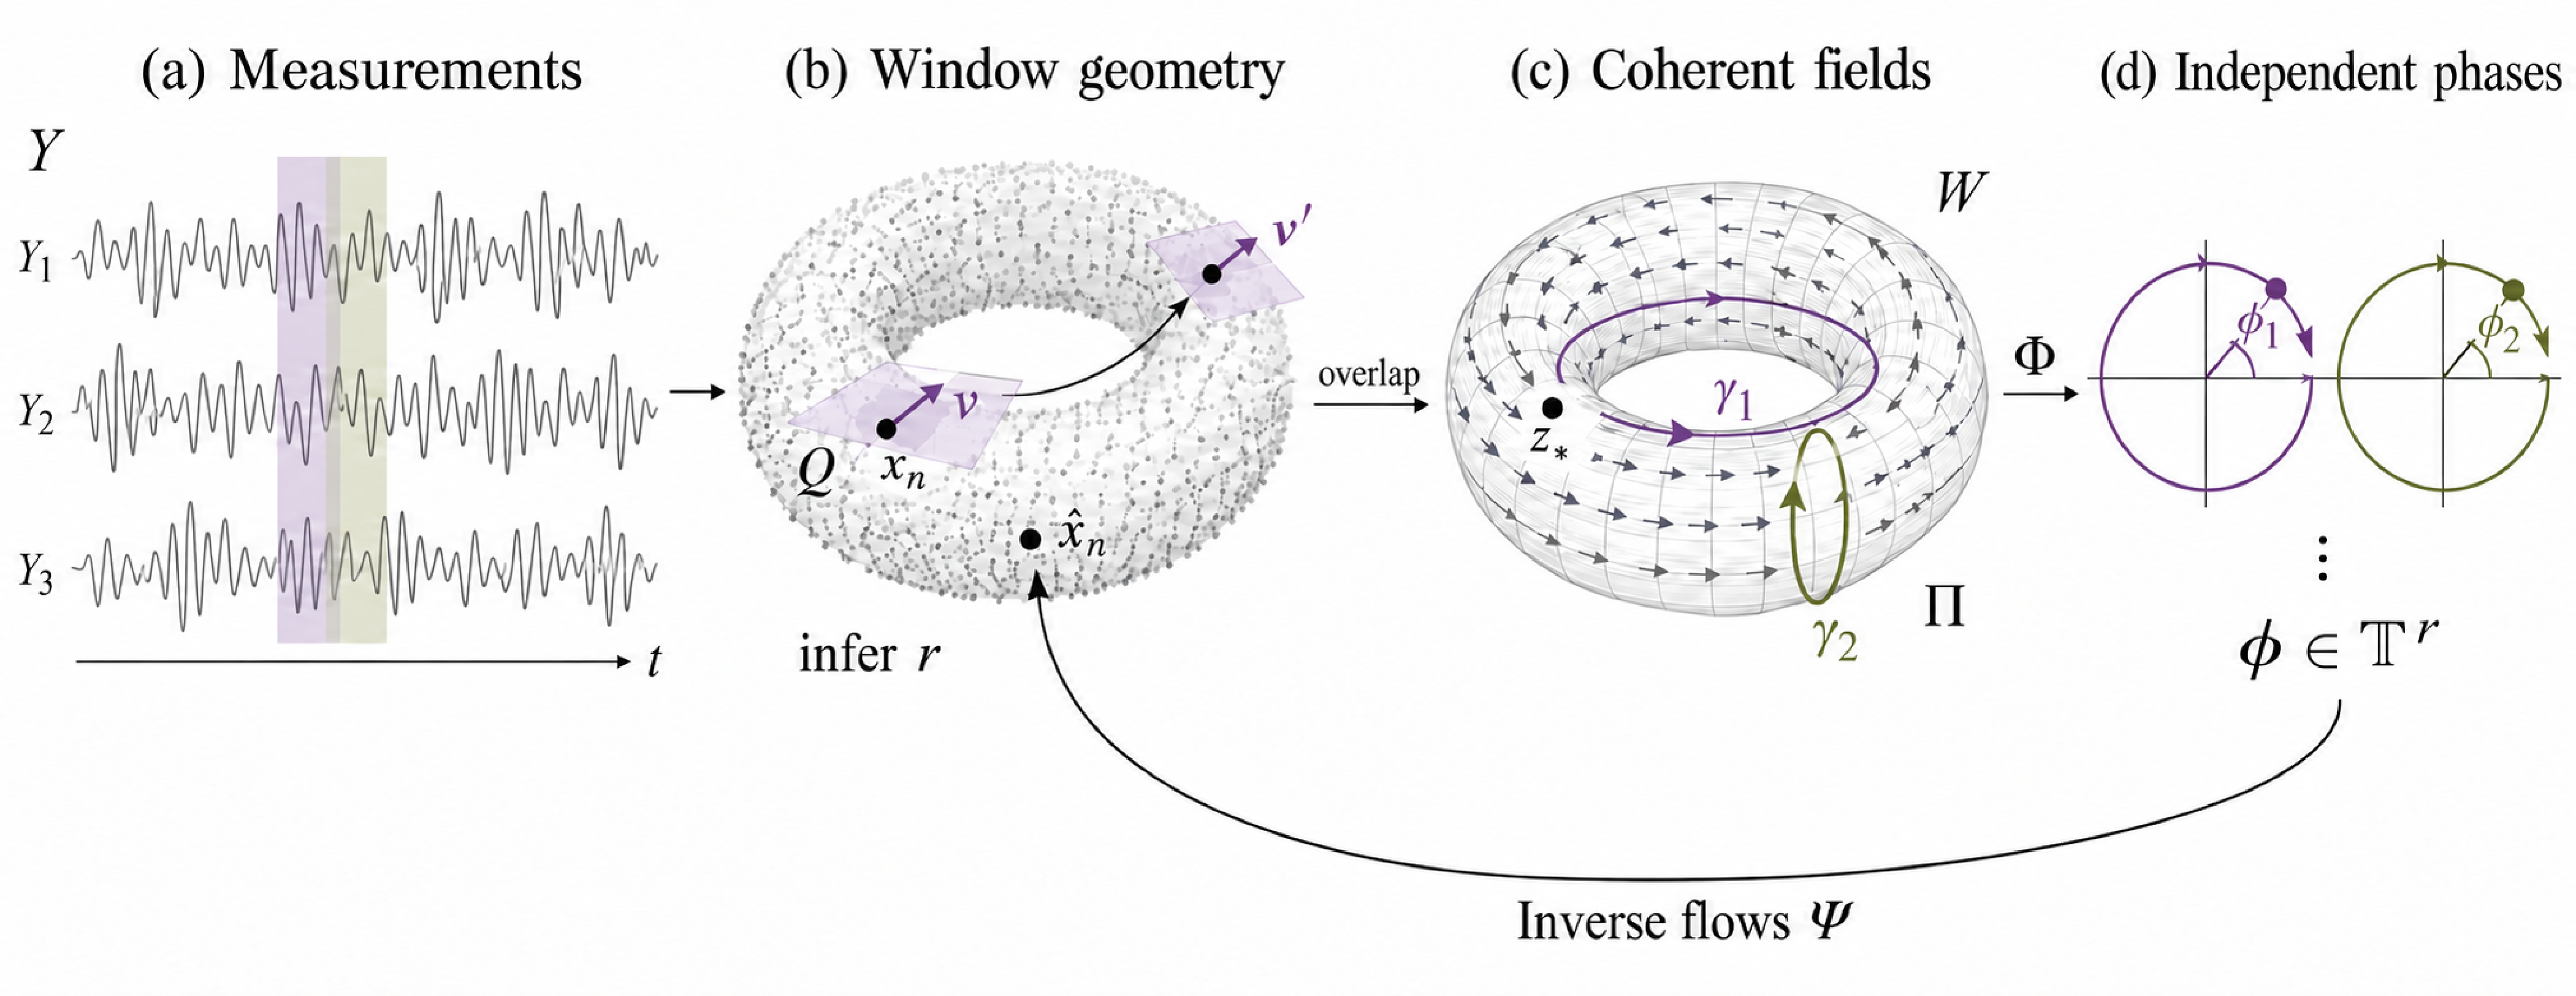
\includegraphics[width=\linewidth]{figures/phase_recovery_objective_violet_olive.pdf}
\caption{From sensor readings to independent phases and back.
The illustrated torus has $r=2$; the method estimates $r$ from the windows.}
\label{fig:phase-recovery-objective}
\end{figure}

\subsection*{1. Windows and tangent geometry}
Each window describes several consecutive readings from all sensors.
From the resulting point cloud, we estimate the number of phases and the
local directions in which windows can move.
\begin{itemize}
\setlength{\itemsep}{2pt}
\item \textbf{Prepare windows.}
Denoise by MSSA~\citep{GrothGhil2011}, subtract a locally smoothed
trend~\citep{SavitzkyGolay1964}, then centre and scale each channel.
Retain the trend for reconstruction. Stack $L$ readings into $x_n^{\mathrm p}$.
Filter settings and candidate window lengths are listed in
\hyperref[app:preparation]{Appendix A.1}.
\item \textbf{Reduce coordinates.}
SVD of the $K_{\mathrm p}$ prepared training windows gives
\[
\widetilde x_n=U_D^\top x_n^{\mathrm p}\in\R^D,
\qquad U_D\in\R^{mL\times D},\quad U_D^\top U_D=I_D.
\]
Truncate at a clear singular-value gap only if the reconstruction error
is small and the estimated local dimension is preserved.
Otherwise retain the numerical span. Write $\widetilde z=U_D^\top z$.
\item \textbf{Estimate $r$.}
Centre neighbouring windows and apply SVD. A gap between large and small
singular values proposes $r$. Under the torus model, each independent
phase also contributes one full-turn cycle. We therefore test this count
on the whole cloud:
\begin{enumerate}
\setlength{\itemsep}{1pt}
\item Starting with the first window, repeatedly select the window farthest
from the selected set. Call these representative windows
$z_v\in\R^{mL}$ \emph{landmarks}; use their reduced coordinates
$\widetilde z_v=U_D^\top z_v$ to measure distances.
\item Join landmarks at distance below $t$ and fill every triangle whose
three edges are present. Filling triangles removes small loops created
by neighbour connections; their boundaries do not count as full phase turns.
\item Count independent graph cycles and remove combinations of triangle
boundaries, using matrix ranks. For example, the outline of two adjacent
triangles is also filled: their shared edge cancels.
\end{enumerate}
Increase $t$ and track the remaining cycles~\citep{deSilva2011,Bauer2021}.
Require an interval with exactly $r$ cycles. Choose $t$ within it so that
balls of radius $t/2$ around the landmarks cover the training windows.
If local SVD is inconclusive, use the group of
cycles with clearly longer lifetimes than the rest. Refine the landmark
set if needed; keep the selected windows, edges and triangles.
$D$ counts linear coordinates; $r$ counts phases.
\item \textbf{Fit tangent planes.}
Fit quadratic constraints $g_a(\widetilde z)\approx0$, validated on withheld
windows. Tangent velocities satisfy
\[
\nabla g_a(\widetilde z)^\top\widetilde v\approx0,
\qquad \widetilde v\in\R^D.
\]
If the solution space is not stably $r$-dimensional, differentiate local
cubic surface fits~\citep{Levin2004,AamariLevrard2019}.
\end{itemize}
This gives orthonormal bases $\widetilde Q(\widetilde z)\in\R^{D\times r}$
and $Q_n=U_D\widetilde Q(\widetilde x_n)\in\R^{mL\times r}$.
Keep the fitted geometry fixed.
The surface fits are specified in \hyperref[app:tangents]{Appendix A.2}.

\begin{figure}[htbp]
\centering
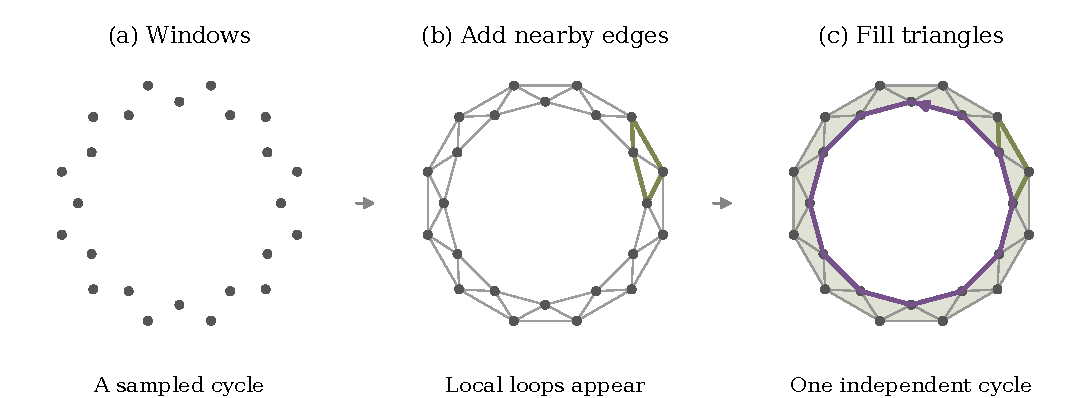
\includegraphics[width=\linewidth]{figures/cycle_count_violet_olive.pdf}
\caption{Why triangles matter. A schematic cloud around a circle.
Neighbour connections create small loops (olive); filling their triangles
leaves one independent cycle around the centre (purple).
The graph is identical in (b) and (c).}
\label{fig:cycle-count}
\end{figure}

\subsection*{2. Overlap transport and coherent fields}
Local tangent bases can have different orientations at different windows.
Matching changes in their shared readings aligns them into fields that
represent the same phase changes along the record.
Define
\[
P_0=\begin{bmatrix}I_{m(L-1)}&0\end{bmatrix},\qquad
P_1=\begin{bmatrix}0&I_{m(L-1)}\end{bmatrix},\qquad
P_0,P_1\in\R^{m(L-1)\times mL},
\]
with $m$ columns in each zero block. These matrices select the shared
readings: $P_0x_{n+1}^{\mathrm p}=P_1x_n^{\mathrm p}$.
Require $\operatorname{rank}D(P_0h_L^{\mathrm p})=r$, so the overlap retains
every tangent direction.

\textbf{Transport.} Match tangent changes on the shared readings:
\[
A_n=\mathop{\arg\min}_{A\in\R^{r\times r}}
\|P_0Q_{n+1}A-P_1Q_n\|_F^2.
\]
Then $Q_na$ is transported to $Q_{n+1}A_na$ for $a\in\R^r$.
Full column rank of $P_0Q_{n+1}$ makes $A_n$ unique.

\textbf{Joint fit.} Fit $r$ tangent fields $W(z)\in\R^{mL\times r}$.
The matrix $R_n$ gives their coefficients in the local basis $Q_n$:
\[
W_n:=W(x_n^{\mathrm p})=Q_nR_n,\qquad
R_{n+1}\approx A_nR_n,\quad R_0=I_r,\quad R_n\in\R^{r\times r}.
\]
The initial basis prevents a zero solution.
Blend local affine predictions and project onto the tangent planes.
Fit their coefficients together~\citep{Thunberg2015}, penalizing transport
errors, disagreement at nearby windows and large coefficients.
Freeze $W$, including its values between observations.
\hyperref[app:field-model]{Appendix A.3} gives the field model and fitting objective.

\subsection*{3. Coefficients of motion}
Express motion as a combination of the fitted field directions.
Integrating these coefficients along a path measures accumulated motion
in one common basis.
For a displacement $v\in\R^{mL}$ at $z$, solve for its frame coefficients
$a=\beta_z(v)\in\R^r$:
\[
(W(z)^\top W(z))a=W(z)^\top v.
\]
For tangent $v$, this gives $v=W(z)a$.
The ideal shift
$T(h_L^{\mathrm p}(\theta))=h_L^{\mathrm p}(\theta+\alpha)$ satisfies
\[
DT_{h_L^{\mathrm p}(\theta)}Dh_L^{\mathrm p}(\theta)
=Dh_L^{\mathrm p}(\theta+\alpha).
\]
Since $Dh_L^{\mathrm p}$ spans the tangent space, exact transport preserves
one invertible matrix $B\in\R^{r\times r}$ along the dense orbit;
continuity gives
\[
W(h_L^{\mathrm p}(\theta))=Dh_L^{\mathrm p}(\theta)B,
\qquad \beta_{h_L^{\mathrm p}(\theta)}Dh_L^{\mathrm p}(\theta)=B^{-1}.
\]
Thus ideal cycle integrals measure full phase turns in the coordinates of $W$.

\subsection*{4. Full periods}
A full turn returns to the same window but has a nonzero integral of
$\beta$. The columns of $\Pi$ record these integrals for $r$ independent
turns. Use the same landmarks, edges and triangles as in step 1.
\begin{enumerate}
\setlength{\itemsep}{2pt}
\item \textbf{Identify full turns.}
Assign integer edge labels $c_{uv}\in\Z^r$ using persistent
cohomology~\citep{deSilva2011}. Their sum along a closed path counts its
signed turns. Filled triangles contribute zero:
\[
c_{vu}=-c_{uv},\qquad c_{uu}=0,\qquad c_{uv}+c_{vw}-c_{uw}=0.
\]
Verify that every unit turn vector $e_j$ occurs as a closed-path sum.
\item \textbf{Measure motion between landmarks.}
For each landmark edge $u\to v$, find a shortest path in a nearest-neighbour
graph of training windows, restricted to the covering balls.
Its labels, added whenever the covering ball changes, must sum
to $c_{uv}$. Compute $b_{uv}=\int_{u\to v}\beta\in\R^r$ using the fixed $W$.
\item \textbf{Fit the full periods.}
Represent each integral as an endpoint difference plus full turns:
$b_{uv}\approx f_v-f_u+\Pi c_{uv}$.
The landmark coordinates $f_v\in\R^r$ and period matrix
$\Pi\in\R^{r\times r}$ are unknown. Find them by least squares:
\[
\min_{\{f_v\},\Pi}\sum_{u\to v}
\|b_{uv}-(f_v-f_u+\Pi c_{uv})\|^2,\qquad f_0=0.
\]
Along a closed path, the endpoint differences cancel. Thus the fitted
integrals $\bar b_{uv}=f_v-f_u+\Pi c_{uv}$ sum to zero around a triangle
and to $\Pi_{:,j}$ for one turn in direction $j$~\citep{Jiang2011}.
The field $W$ remains fixed.
\item \textbf{Choose a shorter period basis.}
Use the lattice-reduction step of toroidal coordinates
(TC)~\citep{Scoccola2023} to choose shorter integer combinations of cycles.
Measure their length through the average squared window motion:
\[
\mathcal G=\Pi^\top\left(K_{\mathrm p}^{-1}\sum_n W_n^\top W_n\right)\Pi.
\]
For a turn vector $c$, $c^\top\mathcal Gc$ is the average of
$\|W_n\Pi c\|^2$. For the resulting $U\in\Z^{r\times r}$ with $\det U=\pm1$, replace
$\Pi\leftarrow\Pi U$ and $c_{uv}\leftarrow U^{-1}c_{uv}$.
This shortens the basis without changing the period lattice.
\end{enumerate}
\hyperref[app:topology]{Appendix A.4} specifies the integer-label
construction and the paths used for integration.

\begin{figure}[htbp]
\centering
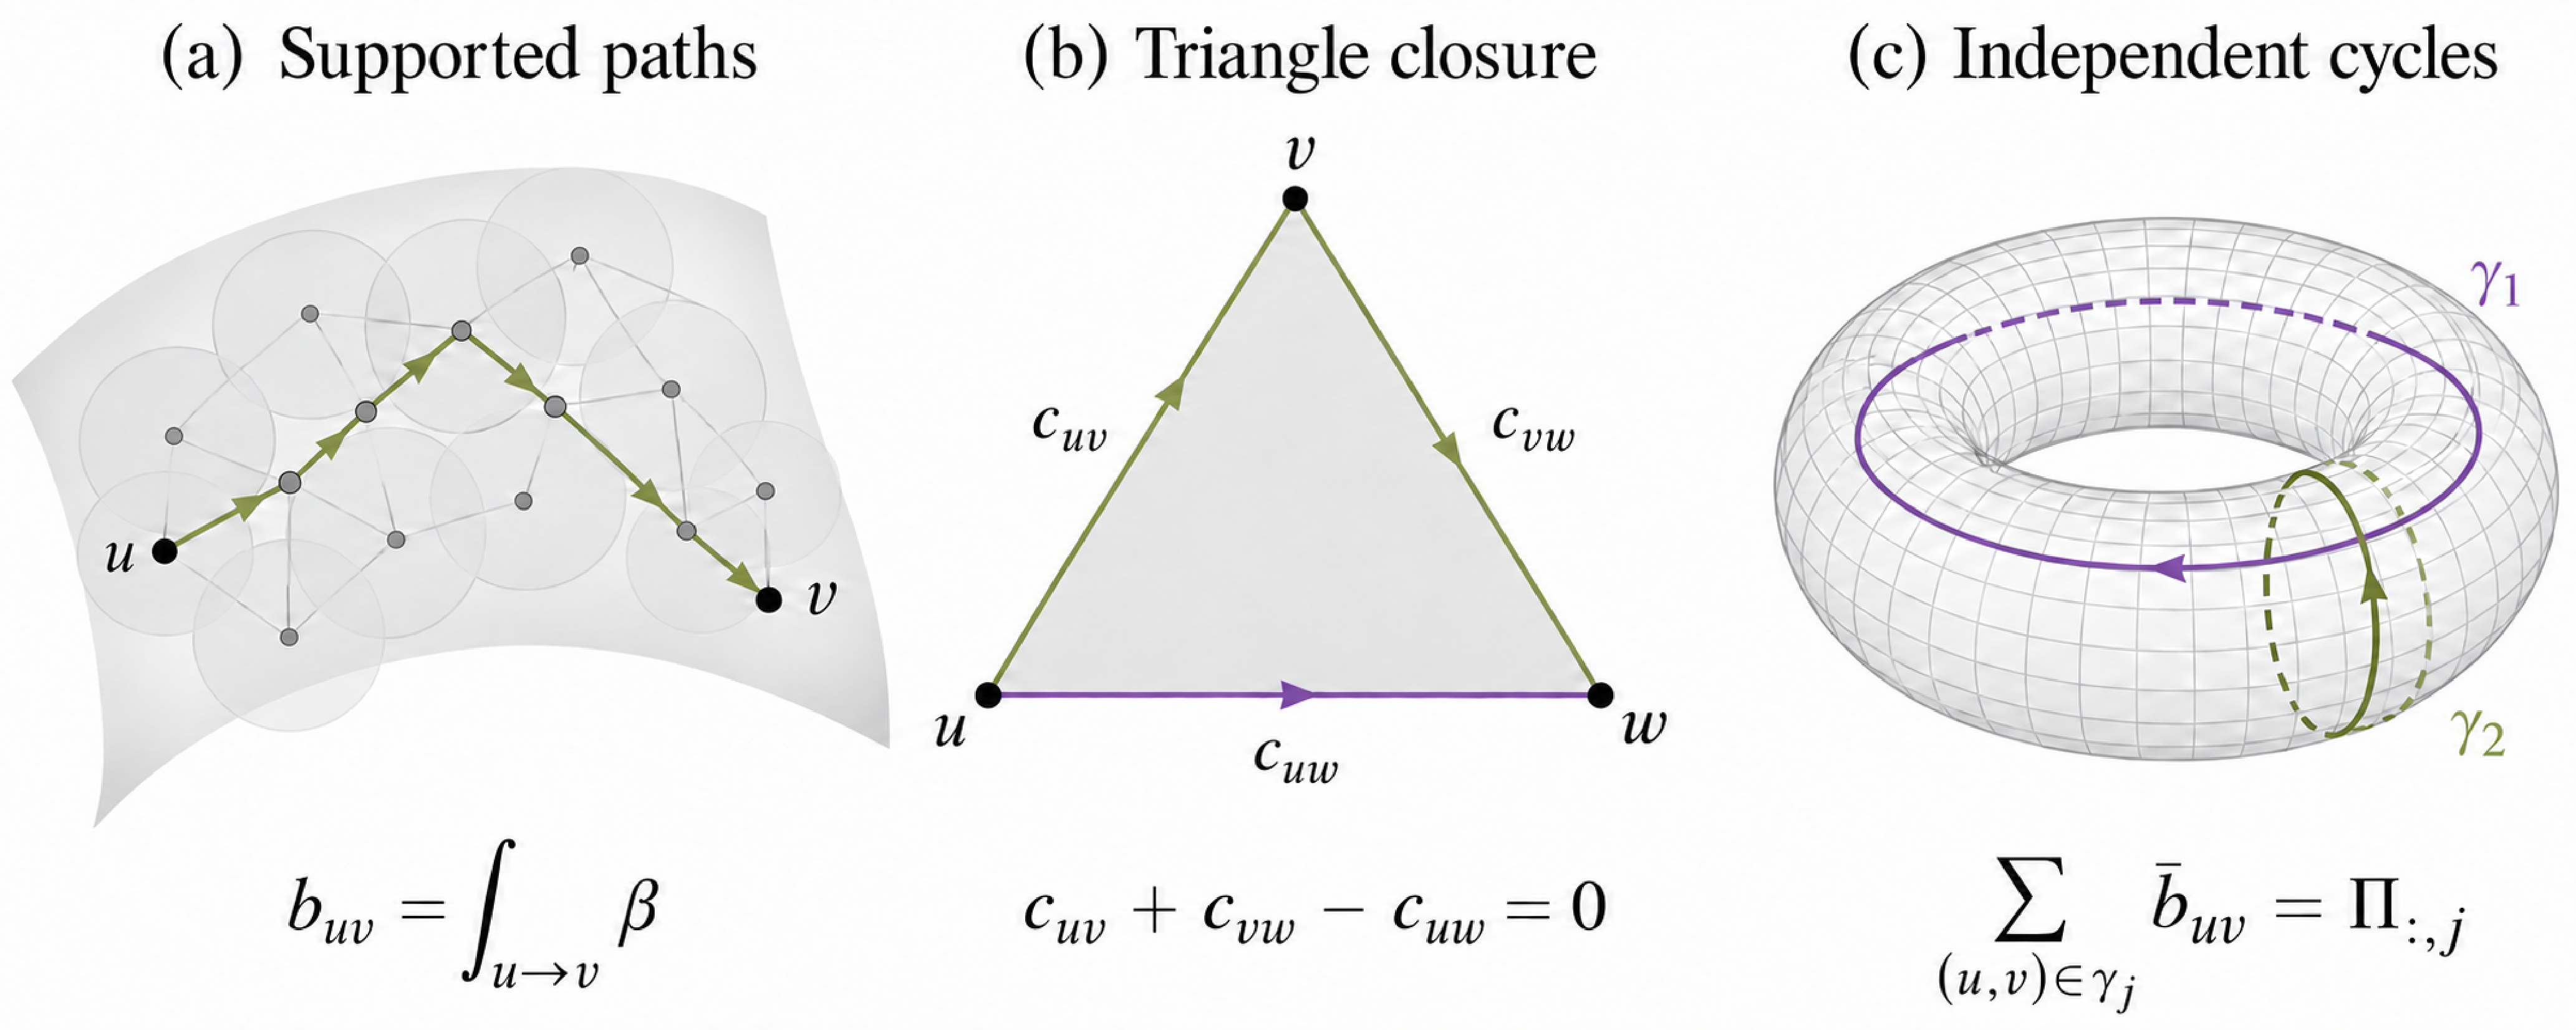
\includegraphics[width=\linewidth]{figures/paths_and_cycles_violet_olive.pdf}
\caption{Paths, triangle closure and independent cycles.
Paths respect the cover and edge labels; corrected cycle integrals give
the columns of $\Pi$. The illustrated torus has $r=2$.}
\label{fig:paths-cycles}
\end{figure}

\subsection*{5. Phase coordinates}
The periods convert accumulated motion into angles. Assign values to the
landmark windows and extend them to nearby windows using the fitted fields.
At each $z_v$, set $q_v=\Pi^{-1}f_v$ (full turns).
For a nearby window $z$, estimate
\[
q_v+\Pi^{-1}\beta_{z_v}(z-z_v).
\]
Local estimates may differ by whole turns, so align them before averaging.
Add the integer turns $c_{uv}$,
where $u$ is any contributing landmark~\citep{Perea2020}:
\[
\Phi(z)=2\pi\sum_{v:\rho_v(z)>0}\rho_v(z)
\left[q_v+c_{uv}+\Pi^{-1}\beta_{z_v}(z-z_v)\right]
-\varphi_{\mathrm{ref}}\pmod{2\pi}.
\]
The smooth weights $\rho_v\ge0$ sum to one, vanish outside their landmark
balls and reproduce each landmark value and derivative.
\hyperref[app:phase-weights]{Appendix A.5 (Phase interpolation)} gives
the weights as functions of distance and defines their values at landmarks.
Contributing landmarks form filled triangles, so the angles are independent of $u$.

\textbf{Phase origin.}
Initially take $z_*=x_0^{\mathrm p}$ as the reference window.
The constant vector $\varphi_{\mathrm{ref}}\in\R^r$ is the value of the
weighted sum, including $2\pi$, at $z_*$. Subtracting it sets $\Phi(z_*)=0$.

Use this fixed map for training and new windows; reject points outside the cover.
It approximates the ideal integral
\[
\Phi(z)=2\pi\Pi^{-1}\int_{z_*}^z\beta\pmod{2\pi}.
\]

\subsection*{6. Inverse reconstruction}
Recover a window by starting at a reference window and changing each phase
by its prescribed amount. Then combine overlapping windows to recover
the sensor record.
Ideally, $\beta W=I_r$ and $D\Phi=2\pi\Pi^{-1}\beta$.
To change only phase $j$ at unit speed, solve
\[
2\pi\Pi^{-1}a=e_j
\quad\Longrightarrow\quad
E_j(z)=W(z)a=\frac{1}{2\pi}W(z)\Pi e_j.
\]
These fields commute in the exact model~\citep{Giannakis2019}.
Starting at $u_0=z_*$, reconstruct by successive flows~\citep[Theorem~9.46]{Lee2012}:
\[
\frac{dw_j}{ds}=E_j(w_j(s)),\qquad w_j(0)=u_{j-1},\qquad
u_j=w_j(\varphi_j),\qquad \Psi(\varphi)=u_r,\quad j=1,\ldots,r.
\]
Evaluate the fixed $W$ along each flow.
For local cubic geometry, failed training reconstruction or full-turn tests trigger
normal corrections back to the same fitted surface.
Rescale $\widehat x_n^{\mathrm p}=\Psi(\varphi_n)$, average copies of each
sensor reading across overlapping windows~\citep{GrothGhil2011}, and
restore the trend to obtain $\widehat Y$.
Integration settings and acceptance thresholds are listed in
\hyperref[app:reconstruction]{Appendix A.6}.

\FloatBarrier
\begin{algorithm}[H]
\caption{TorusFlow}
\small
\textbf{Input:} sensor readings $Y$, sampling interval $\Delta t$.\\
\textbf{Output:} $r$, $\Phi$, $E_j$, $\Psi$, $\widehat Y$, or \texttt{unresolved}.\\
Skip candidates with unresolved geometry or deficient required ranks.
\par\smallskip
\begin{tabular}{@{}r@{\quad}p{0.92\linewidth}@{}}
1 & Denoise; subtract and retain the trend.\\
2 & \textbf{for each} candidate window length and neighbourhood size \textbf{do}\\
3 & \quad Scale signals; build windows; apply SVD; estimate $r$; fit tangent planes.\\
4 & \quad Compute overlap transfers and jointly fit the fields $W$.\\
5 & \quad Label cycles; integrate $\beta$ along supported graph paths.\\
6 & \quad Fit and reduce the period basis $\Pi$; construct $\Phi$ and $E_j$.\\
7 & \quad Integrate $E_j$ to obtain $\Psi$; average windows and restore the trend.\\
8 & \quad \textbf{return} the fit if ranks, phase consistency and reconstruction pass.\\
9 & \quad Otherwise continue with the next candidate.\\
10 & \textbf{end for}; \textbf{return} \texttt{unresolved}.\\
\end{tabular}
\end{algorithm}

\section*{Related methods}

\begin{table}[H]
\centering
\caption{Methods for phase reconstruction.}
\label{tab:method-comparison}
\begingroup
\normalsize
\setlength{\tabcolsep}{6pt}
\setlength{\parskip}{0pt}
\renewcommand{\arraystretch}{1.15}
\begin{tabular}{@{}
  >{\raggedright\arraybackslash}p{0.23\linewidth}
  >{\raggedright\arraybackslash}p{0.33\linewidth}
  >{\raggedright\arraybackslash}p{\dimexpr0.44\linewidth-4\tabcolsep\relax}
  @{}}
\toprule
\textbf{Method} & \textbf{Strengths} & \textbf{Limitations} \\
\midrule
SSA / MSSA\par
\citep{BroomheadKing1986,GrothGhil2011}
& Separates oscillatory modes and reconstructs readings.
& Linear rank counts harmonics as well as phases. \\
\addlinespace[8pt]
Circular coordinates (CC)\par
\citep{deSilva2011}
& Maps independent loops in a point cloud to angles.
& Phase speed can vary; inversion needs another model. \\
\addlinespace[8pt]
Toroidal coordinates (TC)\par
\citep{Scoccola2023}
& Reduces correlation between circular coordinates.
& Phase speed can vary; inversion needs another model. \\
\addlinespace[8pt]
Koopman methods\par
\citep{Giannakis2019}
& Finds dynamical phases and fields; supports reconstruction and forecasting.
& Needs basis truncation, regularization and phase selection. \\
\addlinespace[8pt]
TorusFlow
& Estimates $r$ and phase fields; reconstructs readings using their flows.
& Assumes observable torus dynamics; needs sample coverage and consistent fields. \\
\bottomrule
\end{tabular}
\endgroup
\end{table}

\section*{Experiments}
All fits use sensor readings only; the number of phases is estimated.
We fit on the first part of each record and reconstruct a later observed
block.

\subsection*{Signals and sensors}
\begin{enumerate}
\setlength{\itemsep}{4pt}
\item \textbf{Sine toy: one sensor, one phase.}
The sensor records $y(t)=\sin t$ at $\Delta t=0.4$, without noise or trend.
This is a scalar record with no specified spatial position.
\item \textbf{Two-wave toy: twelve sensors, two phases.}
Sensors at fixed positions $\xi_s\in[0,1]^2$ record two travelling waves:
\[
y_s(n)=\cos(\theta_{n,1}-k_1^\top\xi_s)
       +0.6\cos(\theta_{n,2}-k_2^\top\xi_s),
\qquad
k_1=2\pi(1,0.5)^\top,\quad k_2=2\pi(-0.4,1.1)^\top.
\]
We test clean readings and readings with a quadratic trend and $5\%$ noise.
The wave vectors $k_1,k_2$ give the propagation directions.
\item \textbf{Nonlinear signal: one sensor, one phase.}
The sensor records
\[
y(n)=\exp(0.4\cos\theta_n)+0.25\sin\theta_n+0.15\cos(2\theta_n),
\]
with a linear trend and $10\%$ noise.
\item \textbf{Curved torus: four channels, three phases.}
For phases $(a,b,c)$, the readings are
\[
y=\bigl((2+\cos c)\cos a,\ (2+\cos c)\sin a,
        (2+\sin c)\cos b,\ (2+\sin c)\sin b\bigr)^\top.
\]
The third phase changes the amplitudes of the first two.
We test $0$, $1$, $5$ and $10\%$ noise, without a trend.
These four channels are synthetic observables with no assigned spatial positions.
\end{enumerate}

\begin{figure}[htbp]
\centering
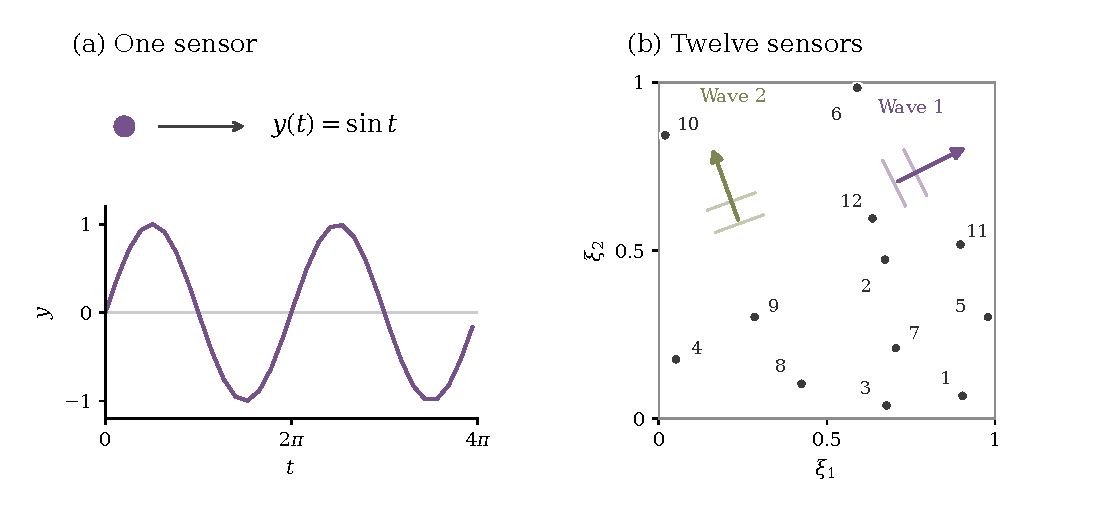
\includegraphics[width=\linewidth]{../experiments/figures/toy_sensors.pdf}
\caption{Toy measurements. Left: one recorded sinusoid.
Right: the actual twelve sensor positions; arrows and wavefronts show
how the two plane waves propagate.}
\label{fig:toy-sensors}
\end{figure}

\subsection*{Evaluation}
We use two errors; smaller values are better.
\begin{itemize}
\item \textbf{Phase error (radians):} the mean angular distance to the reference,
\[
E_\varphi=\operatorname{mean}_{n,j}
\left|\operatorname{Arg}e^{i(\varphi_{n,j}-\theta^{\rm ref}_{n,j})}\right|.
\]
The reference $\theta^{\rm ref}$ accounts for phase ordering, orientation
and origin, fitted on training data only. $\operatorname{Arg}\in(-\pi,\pi]$.
\item \textbf{Signal error (percent):} $100E_Y$, where
\[
E_Y=\sqrt{\operatorname{mean}_{n,s}
\left(\frac{\widehat Y_{s,n}-Y^0_{s,n}}{\sigma_s}\right)^2}.
\]
Here $Y^0$ is the clean signal including the trend, and $\sigma_s$ is the
standard deviation of the clean oscillatory training signal at sensor $s$.
\end{itemize}
Phase errors use complete test windows; signal errors use retained test
samples. Gaussian noise percentages are relative to the same $\sigma_s$.
\hyperref[app:evaluation]{Appendix A.7} lists the data splits and scored samples.

\subsection*{Results}
Each row is one realization; the four curved-torus runs use the same
orbit and scaled noise.

% BEGIN RESULTS_TABLE
\begin{table}[H]
\centering\small
\setlength{\tabcolsep}{6pt}
\begin{tabular}{lrrrrr}
\toprule
Signal & Sensors & Noise (\%) & $\widehat r$ & Phase error (rad) & Signal error (\%) \\
\midrule
Sine toy & 1 & 0 & 1 & 0.00020 & 0.496 \\
Two-wave toy & 12 & 0 & 2 & 0.00134 & 0.110 \\
One nonlinear sensor & 1 & 10 & 1 & 0.01157 & 2.499 \\
Two waves & 12 & 5 & 2 & 0.00431 & 0.695 \\
Curved torus & 4 & 0 & 3 & 0.00439 & 0.456 \\
Curved torus & 4 & 1 & 3 & 0.00933 & 0.650 \\
Curved torus & 4 & 5 & 3 & 0.01091 & 1.840 \\
Curved torus & 4 & 10 & 3 & 0.01393 & 2.285 \\
\bottomrule
\end{tabular}
\caption{TorusFlow results. $\widehat r$ is the estimated phase count.
True phase counts are $1$ for scalar signals, $2$ for two waves and $3$
for the curved torus.}
\label{tab:experiment-results}
\end{table}

% END RESULTS_TABLE

\begin{figure}[H]
\centering
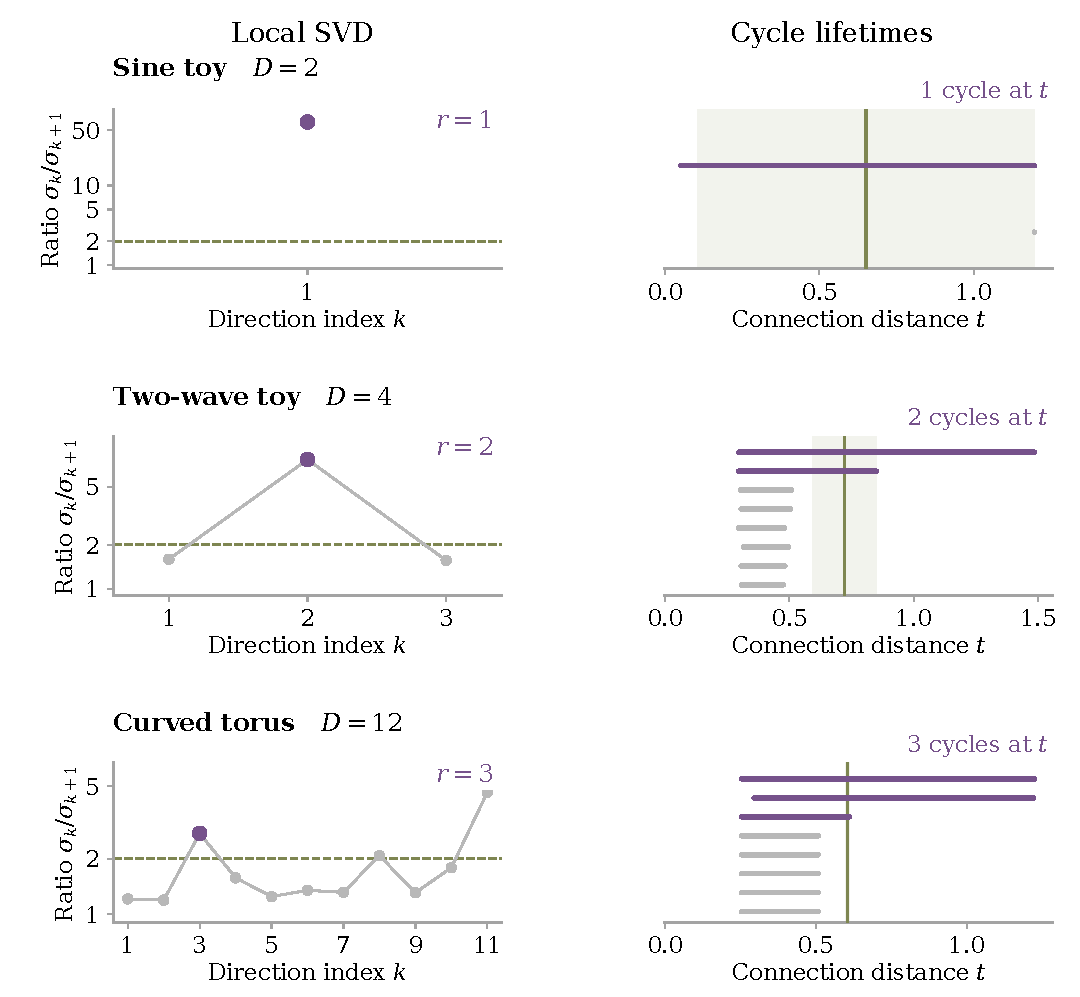
\includegraphics[width=\linewidth]{../experiments/figures/dimension_selection.pdf}
\caption{Choosing $r$ in three noise-free examples.
Left: the first median local singular-value ratio $\sigma_k/\sigma_{k+1}\ge2$
proposes $r$ (purple).
Right: bars show cycle lifetimes; the chosen $t$ (olive) crosses exactly
$r$ bars; shading marks the accepted interval.
Up to eight longest lifetimes are displayed; all cycles enter
the count. Balls of radius $t/2$ cover all training windows.}
\label{fig:dimension-selection}
\end{figure}

\begin{figure}[htbp]
\centering
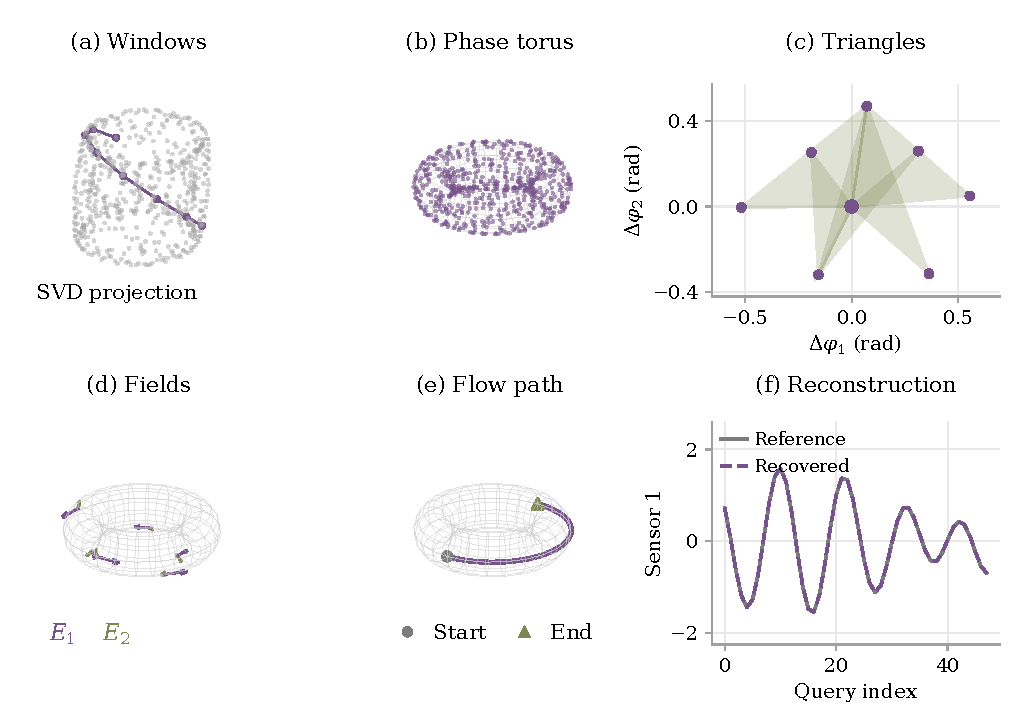
\includegraphics[width=\linewidth]{../experiments/figures/toy_walkthrough.pdf}
\caption{TorusFlow on the clean two-wave toy.
(a) Window coordinates from SVD. (b) Recovered phases displayed on a torus.
(c) Six triangles from the fitted complex. (d) Estimated phase fields.
(e) A path obtained by integrating the first field.
(f) Reconstruction at sensor~1.
The torus displays phase coordinates; sensor positions are shown in Figure~\ref{fig:toy-sensors}.}
\label{fig:toy-walkthrough}
\end{figure}

\begin{figure}[htbp]
\centering
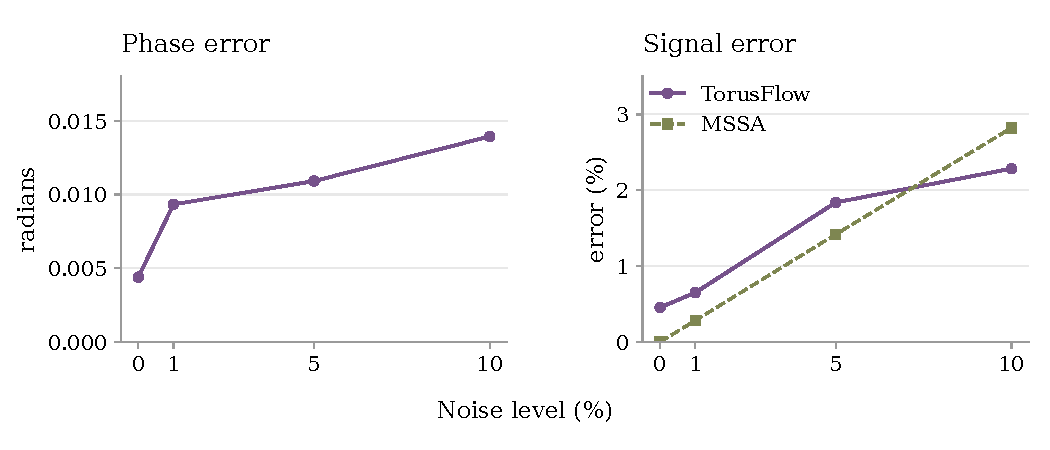
\includegraphics[width=\linewidth]{../experiments/figures/experiments_curved_noise.pdf}
\caption{Noise sensitivity on the three-phase torus.
Left: phase error of TorusFlow. Right: signal error of TorusFlow and MSSA.}
\label{fig:experiment-noise}
\end{figure}

\subsection*{Comparison}
SSA/MSSA~\citep{BroomheadKing1986,GrothGhil2011}, circular coordinates
(CC)~\citep{deSilva2011} and toroidal coordinates
(TC)~\citep{Scoccola2023} receive the same raw inputs and are evaluated
at the same times. The two cases are the nonlinear single-sensor signal
with $10\%$ noise and the two-wave signal with $5\%$ noise, including their trends.
A $+$CDF variant rescales its angles using their training empirical
distribution. A dash denotes an output that was not evaluated or, for
Koopman phases, a failed complete primitive phase-basis check.

% BEGIN BASELINES_TABLE
\begin{table}[H]
\centering\small
\setlength{\tabcolsep}{9pt}
\begin{tabular}{lrrrr}
\toprule
& \multicolumn{2}{c}{Phase error (rad)} & \multicolumn{2}{c}{Signal error (\%)}\\
\cmidrule(lr){2-3}\cmidrule(lr){4-5}
Method & Nonlinear & Two waves & Nonlinear & Two waves\\
\midrule
TorusFlow & 0.01157 & 0.00431 & 2.499 & 0.695 \\
SSA & -- & -- & 3.753 & 1.728 \\
MSSA & -- & -- & 3.753 & 0.702 \\
CC & 0.38152 & 0.11481 & -- & -- \\
TC & 0.38152 & 0.12429 & -- & -- \\
CC+CDF & 0.00983 & 0.08566 & -- & -- \\
TC+CDF & -- & 0.09174 & -- & -- \\
Koopman & -- & 0.06271 & 2.299 & 5.430 \\
\bottomrule
\end{tabular}
\caption{Comparison on the same test inputs and evaluated times.
The nonlinear and two-wave cases use $10\%$ and $5\%$ noise, respectively.
CDF calibration uses training data only.}
\label{tab:experiment-baselines}
\end{table}

% END BASELINES_TABLE

% BEGIN KOOPMAN_TABLE
\begin{table}[H]
\centering\small
\setlength{\tabcolsep}{5pt}
\begin{tabular}{lrrrrrr}
\toprule
& & & \multicolumn{2}{c}{Phase error (rad)} & \multicolumn{2}{c}{Signal error (\%)}\\
\cmidrule(lr){4-5}\cmidrule(lr){6-7}
Signal & Noise (\%) & $\widehat r_{\rm K}$ & TorusFlow & Koopman & TorusFlow & Koopman\\
\midrule
Sine toy & 0 & 1 & 0.00020 & 0.00778 & 0.496 & 0.981 \\
Two-wave toy & 0 & 2 & 0.00134 & 0.06535 & 0.110 & 5.373 \\
One nonlinear sensor & 10 & 2 & 0.01157 & -- & 2.499 & 2.299 \\
Two waves & 5 & 2 & 0.00431 & 0.06271 & 0.695 & 5.430 \\
Curved torus & 0 & 3 & 0.00439 & -- & 0.456 & 3.914 \\
Curved torus & 1 & 3 & 0.00933 & -- & 0.650 & 3.549 \\
Curved torus & 5 & 3 & 0.01091 & -- & 1.840 & 3.583 \\
Curved torus & 10 & 3 & 0.01393 & -- & 2.285 & 3.915 \\
\bottomrule
\end{tabular}
\caption{Koopman baseline~\citep{Giannakis2019} on all eight identical test blocks.
$\widehat r_{\rm K}$ is the number of selected Koopman phases.
A dash marks an incomplete or nonprimitive phase basis; signal reconstruction
uses the full spectral basis and can still be evaluated.
Implementation: \hyperref[app:koopman]{Appendix A.8}.}
\label{tab:experiment-koopman}
\end{table}

% END KOOPMAN_TABLE

\clearpage
\section*{Appendix A. Implementation details}
\phantomsection\label{app:numerics}
\begingroup\small
\setlength{\parskip}{3pt}
\setlength{\topsep}{3pt}
\setlength{\partopsep}{0pt}
\setlength{\abovedisplayskip}{4pt}
\setlength{\belowdisplayskip}{4pt}

\subsection*{A.1. Preparation and candidate search}
\phantomsection\label{app:preparation}
These settings define signal preparation and the search over window lengths
and neighbourhood sizes.
\begin{center}
\begin{tabular}{@{}p{0.34\linewidth}p{0.61\linewidth}@{}}
\toprule
Operation & Setting\\
\midrule
MSSA & Lag $32$; rank at most $24$, selected by masked cross-validation.
Mask every delay copy of each held-out measurement.\\
Trend filter & Savitzky--Golay window $129$, degree $2$.\\
Boundary trim & $95$ samples at each end. Keep original timestamps and
reindex the retained block of length $N_{\mathrm p}$.\\
Channel scaling & Replace scales below $10^{-12}$ times the largest by $1$;
reject an entirely constant record.\\
SVD & Relative numerical cutoff $10^{-10}$. Reduce at the largest
consecutive singular-value ratio of at least $10$.\\
Reduction check & Keep the numerical span if the discarded relative norm
exceeds $0.05$ or a resolved local-dimension estimate changes.\\
Window candidates & $L\in\{4,8,16,32,48\}$, subject to $mL\le128$.\\
Neighbour candidates & $k\in\{24,48,96\}$.\\
Field landmarks & At most $64$, chosen by farthest-point sampling
starting at the first training window.\\
\bottomrule
\end{tabular}
\end{center}
Retain the first candidate passing all training checks. Reduction checks
cannot guarantee preservation of arbitrarily weak phase directions.

Let $\mu\in\R^m$ contain training residual means and let diagonal $S$
contain channel scales. Prepared measurements and windows are
\[
y_n^{\mathrm p}=\frac{S^{-1}(y_n^{\mathrm{osc}}-\mu)}{\sqrt{mL}},
\qquad x_n^{\mathrm p}=((y_n^{\mathrm p})^\top,\ldots,
(y_{n+L-1}^{\mathrm p})^\top)^\top,
\qquad K_{\mathrm p}=N_{\mathrm p}-L+1.
\]
Preparation is assumed to preserve the observable phase directions.
Its noiseless observation map $g^{\mathrm p}$ defines the delay map
$h_L^{\mathrm p}$ and $M=h_L^{\mathrm p}(\T^r)$.
Geometry queries at $z\in\R^{mL}$ use $\widetilde z=U_D^\top z\in\R^D$.

\subsection*{A.2. Tangent planes}
\phantomsection\label{app:tangents}
Estimate the $r$ tangent directions by differentiating fitted surface equations.

\textbf{Quadratic fit.}
Use a feature vector $f(\widetilde z)$ containing $1$, all coordinates and
all pairwise products. Fit relations
\[
g_a(\widetilde z)=\widetilde z^\top C_a\widetilde z+
 a_a^\top\widetilde z+b_a,\qquad
C_a=C_a^\top\in\R^{D\times D},\quad a_a\in\R^D,\ b_a\in\R.
\]
Normalize each relation's coefficient vector to unit norm.
Set $G(\widetilde z)_{a,:}=\nabla g_a(\widetilde z)^\top$ and let
$\lambda_1\le\cdots\le\lambda_D$ be the eigenvalues of $G^\top G$.
Exact relations give the tangent plane $\ker G$; approximate relations
use its $r$ smallest right singular directions.
\begin{center}
\begin{tabular}{@{}p{0.34\linewidth}p{0.61\linewidth}@{}}
\toprule
Check & Rule\\
\midrule
Feature budget & $1+D+D(D+1)/2\le\min(K_{\mathrm p}/2,1024)$.\\
Fit/validation split & Fit four fifths of TRAIN; validate on every fifth row.\\
Row residual & $\max_a|g_a(\widetilde z)|/\|f(\widetilde z)\|_2$;
use the maximum over rows.\\
Exact fit, tried first & Relative tolerance $10^{-10}$ and gradient rank
$D-r$ throughout TRAIN, with eigenvalue tolerance $10^{-8}$.\\
Approximate fit & Reuse the feature SVD with cutoffs
$\tau=10^{-4}2^j$, $j=0,\ldots,6$; require fitting and validation
residuals at most $3\tau$.\\
\bottomrule
\end{tabular}
\end{center}
For an approximate fit, require throughout TRAIN
\[
\frac{\lambda_{r+1}}{\lambda_D}\ge10^{-8},\qquad
1-\frac{\lambda_r}{\lambda_{r+1}}\ge0.1.
\]
Choose the cutoff maximizing the worst validation value of
$(\lambda_{r+1}-\lambda_r)/\lambda_D$; break ties in favour of the smaller
cutoff. Check spectral separation and data support at each query.
If the quadratic fit fails, use local cubic surfaces.

\textbf{Local cubic fallback.}
At every retained window $a_i=\widetilde x_i$, fit a polynomial surface:
\begin{enumerate}
\setlength{\itemsep}{1pt}
\item Set $q_g=\binom{r+3}{3}-1$ and use the
$k_g=\min\{K_{\mathrm p}-1,\max(k,q_g+2)\}$ nearest other windows.
Reject if $k_g<q_g$. Write their indices as $\mathcal N_i$ and ordered
distances as $d_{i,j}$.
\item Let $h_g$ be the median positive $d_{i,\min(8,k_g)}$ and set
$\rho_i=\max\{d_{i,k_g},10^{-6}h_g\}$. Reject if $h_g$ is undefined.
PCA of $a_j-a_i$ gives $\widehat Q_i\in\R^{D\times r}$.
\item For $\delta_{ij}=(a_j-a_i)/\rho_i$ and
$u_{ij}=\widehat Q_i^\top\delta_{ij}$, fit a normal polynomial
$p_i:\R^r\to\R^D$ of degrees $1$ through $3$:
\[
\min_{p_i}\sum_{j\in\mathcal N_i}e^{-\|\delta_{ij}\|^2}
\left\|p_i(u_{ij})-
(I_D-\widehat Q_i\widehat Q_i^\top)\delta_{ij}\right\|^2,
\qquad \widehat Q_i^\top p_i\equiv0.
\]
Use least-squares cutoff $10^{-10}$. Twice replace $\widehat Q_i$ by
an orthonormal basis of $\widehat Q_i+Dp_i(0)$ and refit $p_i$.
\end{enumerate}
At a query $\widetilde z$, evaluate
\[
\begin{aligned}
g_i(u)&=a_i+\rho_i\bigl(\widehat Q_i u+p_i(u)\bigr),\\
u_i(\widetilde z)&=\widehat Q_i^\top(\widetilde z-a_i)/\rho_i,
\qquad J_i(\widetilde z)=\widehat Q_i+Dp_i(u_i(\widetilde z)).
\end{aligned}
\]
For $d_i=\|\widetilde z-a_i\|<4h_g$, normalize
\[
w_i(\widetilde z)\propto
\exp\!\left[-\frac{d_i^2}{2h_g^2}
-\frac{d_i^2}{16h_g^2-d_i^2}\right].
\]
Set $w_i=0$ outside this support and reject unsupported queries.
The leading $r$ eigendirections of
\[
\sum_i w_i(\widetilde z)J_i(\widetilde z)
\bigl(J_i(\widetilde z)^\top J_i(\widetilde z)\bigr)^{-1}
J_i(\widetilde z)^\top
\]
define $\widetilde Q$ and $\widetilde P=\widetilde Q\widetilde Q^\top$.
Require an eigenvalue gap greater than $0.1$ after direction $r$.
Differentiate the polynomials, weights and separated spectral projector
analytically. The same charts give the position estimate
$\bar g(\widetilde z)=\sum_iw_i(\widetilde z)g_i(u_i(\widetilde z))$.

\subsection*{A.3. Transported fields}
\phantomsection\label{app:field-model}
Define the field between windows and fit its coefficients from overlap transport.

Compute overlap transport from
\[
(J_n^\top J_n)A_n=J_n^\top P_1Q_n,\qquad A_n\in\R^{r\times r},
\qquad J_n=P_0Q_{n+1}.
\]
At $J$ field landmarks $a_\ell\in\R^D$, use tangent bases
$\widetilde Q_\ell$ and local affine models
\[
\begin{aligned}
u_\ell(\widetilde z)
&=\widetilde Q_\ell^\top(\widetilde z-a_\ell)/h\in\R^r,\\
V_\ell(\widetilde z)
&=\widetilde Q_\ell
\left(M_{\ell0}+\sum_{j=1}^r u_{\ell,j}(\widetilde z)M_{\ell j}\right)
\in\R^{D\times r}.
\end{aligned}
\]
The unknown matrices $M_{\ell j}\in\R^{r\times r}$ specify values
($j=0$) and linear variations ($j\ge1$).
Set $h>0$ to the median TRAIN distance to the fourth nearest field landmark
(or the last available if $J<4$).
Blend the models with normalized Gaussian weights~\citep{MelenkBabuska1996}:
\[
\eta_\ell(\widetilde z)\propto
\exp\!\left(-\frac{\|\widetilde z-a_\ell\|^2}{2h^2}\right),
\qquad \sum_{\ell=1}^J\eta_\ell(\widetilde z)=1.
\]
With $\widetilde P=\widetilde Q\widetilde Q^\top$, project onto the query tangent plane:
\[
\begin{aligned}
\widetilde W(\widetilde z)
&=\widetilde P(\widetilde z)
\left[\mathsf A_0+\sum_{k=1}^D\widetilde z_k\mathsf A_k+
\sum_{\ell=1}^J\eta_\ell(\widetilde z)V_\ell(\widetilde z)\right],\\
W(z)&=U_D\widetilde W(U_D^\top z)\in\R^{mL\times r}.
\end{aligned}
\]
Include the global affine block $\mathsf A_k\in\R^{D\times r}$ only if
$D(D+1)\le Jr(r+1)$; otherwise set it to zero.
Freeze geometry and weights before fitting. At TRAIN windows, set
\[
\widetilde W_n=\widetilde W(\widetilde x_n),\qquad
R_n=\widetilde Q(\widetilde x_n)^\top\widetilde W_n.
\]
Fit all coefficients jointly:
\[
\begin{aligned}
\min_{M,\mathsf A}\quad&
\frac{\sum_{n=0}^{K_{\mathrm p}-2}
\|R_{n+1}-A_nR_n\|_F^2}{(K_{\mathrm p}-1)r}
+\lambda_s\frac{\sum_{n=0}^{K_{\mathrm p}-1}
\|\widetilde W_n-\widetilde W_{\nu(n)}\|_F^2}{K_{\mathrm p}D}\\
&+\frac{\lambda_r}{K_f}\left(
\sum_{\ell=1}^J\sum_{j=0}^r\|M_{\ell j}\|_F^2+
\sum_{k=0}^D\|\mathsf A_k\|_F^2\right),\qquad R_0=I_r.
\end{aligned}
\]
Here $\nu(n)$ is the nearest other training window, $K_f$ counts included
dictionary columns, and $\lambda_s=10^{-3}$, $\lambda_r=10^{-6}$.
The three terms enforce transport, agreement at nearby states and bounded
coefficients.

\subsection*{A.4. Topology and paths}
\phantomsection\label{app:topology}
Select a distance scale that resolves $r$ cycles and covers the training
windows, then construct labelled paths for the period integrals.

Use Ripser for persistence~\citep{Bauer2021} and DREiMac for cocycles and
landmarks~\citep{Perea2023}.

\textbf{Cycle count.}
At distance threshold $t$, let $N_v,N_e,N_c$ be the numbers of vertices,
edges and connected components. The triangle-boundary matrix $\partial_2$
has edges as rows and triangles as columns, with entries $\pm1$ along
each oriented boundary and zero elsewhere. Then
\[
b_1(t)=N_e-N_v+N_c-\operatorname{rank}_{\mathbb F_{47}}\partial_2.
\]
The graph contributes $N_e-N_v+N_c$ independent cycles; triangle boundaries
remove the rank term. Here $\mathbb F_{47}$ denotes arithmetic modulo $47$.
Ripser tracks these cycles across thresholds.
\begin{center}
\begin{tabular}{@{}p{0.34\linewidth}p{0.61\linewidth}@{}}
\toprule
Operation & Setting\\
\midrule
Initial complex & At most $192$ topology landmarks.\\
Refinement & $384$, $768$, $1024$, $1536$, then at most $2048$ landmarks.
Keep the selected resolution for the period complex.\\
Final filtration cap & $1.1$ times the previous common death; if unavailable,
use the RMS norm of $\widetilde x_n$. Use the same cap for periods.\\
Local dimension estimate & At $64$ uniformly selected TRAIN windows,
use $24$ neighbours. The first median consecutive singular-value ratio
at least $2$ proposes $r$.\\
Cocycle arithmetic & Modulo $47$, followed by an integer lift.\\
Path graph & $24$ nearest neighbours, restricted to cover-supported segments.\\
Segment integrals & Three-point Gaussian quadrature, in both directions.\\
\bottomrule
\end{tabular}
\end{center}

\textbf{Choose the dimension and cover.}
Order persistent classes by observed lifetime. For a class surviving the
maximum tested distance (the filtration cap), its death and lifetime
have only lower bounds.
The first $r$ classes must share an interval with $2b<d$, where $b$ is
the latest birth and $d$ the earliest death.
If local geometry supplies no dimension, choose the prefix maximizing the lifetime ratio of the last included
class to the first excluded class, requiring a ratio of at least $2$.
Do not infer a dimension from lifetime ratios involving cycles still
present at that cutoff alone.
Require $1\le r<D$. This dimension rule is a finite-data heuristic.

Let $\epsilon_{\mathrm{land}}$ be the largest distance from TRAIN to its
nearest landmark, and let $\delta$ be half the median positive nearest-neighbour
distance within TRAIN. Split
\[
\max\{2b,\,2(\epsilon_{\mathrm{land}}+\delta)\}<t<d
\]
at persistence births and deaths. Choose the midpoint of the widest
interval with exactly $r$ active classes, strictly below any filtration
cap, and set $a_{\mathrm{cov}}=t/2$.
Use this rule both before field fitting and for the period complex.
The resulting cover contains the $\delta$-neighbourhood of TRAIN;
arbitrary new observations may lie outside it.

\textbf{Check the integer cycles.}
Lift cocycle labels modulo $47$ to integers while preserving triangle
closure; apply signed integer corrections when needed. Require:
\begin{itemize}
\setlength{\itemsep}{1pt}
\item a connected complex covering all training windows;
\item first cohomology dimension exactly $r$ modulo $47$;
\item column Hermite normal form $I_r$ for label sums around the
fundamental cycles of a spanning tree.
\end{itemize}
This certificate applies to the finite complex.

\textbf{Construct integration paths.}
Join topology landmarks by shortest paths on the supported graph.
For quadratic geometry, use verified chords. For local cubic geometry,
use the polynomial path
\[
\gamma_{uv}(s)=
(1-s)g_u\!\left(s\widehat Q_u^\top\Delta/\rho_u\right)
+s\,g_v\!\left((s-1)\widehat Q_v^\top\Delta/\rho_v\right),
\quad \Delta=a_v-a_u,\quad 0\le s\le1,
\]
only if its control polygon lies within one covering ball; otherwise use
a verified chord. Integrate along the fine edges of the selected paths
in both directions. Require their label sums to equal the corresponding
topology-edge labels.

\subsection*{A.5. Phase interpolation}
\phantomsection\label{app:phase-weights}
These weights extend the landmark phase estimates to nearby windows
while preserving the value and derivative at each landmark.
For $d_v=\|U_D^\top(z-z_v)\|$, blend local phase estimates with
\[
\rho_v(z)\propto
\begin{cases}
d_v^{-4}\exp\!\left(-\dfrac{d_v^2}{a_{\mathrm{cov}}^2-d_v^2}\right),
&0<d_v<a_{\mathrm{cov}},\\
0,&d_v\ge a_{\mathrm{cov}},
\end{cases}
\qquad \sum_v\rho_v(z)=1.
\]
Only landmarks within $a_{\mathrm{cov}}$ contribute; nearer landmarks
receive larger weights. At $z=z_v$, set $\rho_v=1$ and all other weights
to zero by continuity. The resulting phase map matches the local estimate
and its derivative at that landmark.

\subsection*{A.6. Acceptance and reconstruction}
\phantomsection\label{app:reconstruction}
The thresholds determine whether a fitted model is accepted.
The integration settings specify how its fields reconstruct windows.

Normalize training flow errors by
$\sigma_x=(K_{\mathrm p}^{-1}\sum_n\|x_n^{\mathrm p}\|^2)^{1/2}$.
Inverse errors include directions discarded by SVD.
\begin{center}
\begin{tabular}{@{}p{0.76\linewidth}r@{}}
\toprule
Diagnostic & Threshold\\
\midrule
Relative edge-integral correction & $0.05$\\
Normalized RMS error in $D\Phi\,E-I_r$ & $0.15$\\
RMS phase-increment error (radians) & $0.05$\\
Relative inverse window error & $0.05$\\
Relative full-turn return defect & $0.05$\\
Relative forward/reverse flow-order discrepancy & $0.05$\\
Relative new-window projection error & $0.10$\\
Relative overlap mismatch before averaging & $0.10$\\
\bottomrule
\end{tabular}
\end{center}
Also require $\sigma_{\min}(J_n)\ge10^{-3}$,
$\operatorname{cond}(\Pi)\le10^8$, full field rank, tangent spectral
separation and coverage. Test inverse reconstruction and flow order at
$16$ uniformly selected TRAIN windows; test full turns from $z_*$.
Use RK4, phase representatives in $(-\pi,\pi]$, a fixed flow order and
angular steps at most $0.12$. Reject a trajectory leaving geometric support.

\textbf{Optional normal correction.}
With local cubic geometry, if ambient inverse reconstruction or the
full-turn test fails, retry with a normal correction after every RK4 step:
\[
\widetilde z\leftarrow\widetilde z+
\bigl(I_D-\widetilde Q(\widetilde z)\widetilde Q(\widetilde z)^\top\bigr)
\bigl(\bar g(\widetilde z)-\widetilde z\bigr).
\]
Here $\bar g$ is the position estimate from the frozen local charts.
This is a geometry-constrained finite inverse; it changes the ambient ODE.
\begin{center}
\begin{tabular}{@{}p{0.34\linewidth}p{0.61\linewidth}@{}}
\toprule
Correction check & Rule\\
\midrule
Normal residual & Below $10^{-9}\sigma_x$ within $20$ iterations;
otherwise reject.\\
Reference point & Correct $z_*$ and reset the phase origin there;
require displacement below $0.05\sigma_x$.\\
Full turns & Test from $8$ training windows.\\
Step selection & Largest step in $\{0.12,0.06,0.03\}$ passing the original
checks and giving a return-point difference below $0.005\sigma_x$
when halved.\\
Constrained phase speed & Central differences with angular increments
$\pm10^{-4}$ at $16$ training windows.\\
\bottomrule
\end{tabular}
\end{center}

\textbf{New observations.}
Repeat coverage, duality, reconstruction and overlap checks. Compare
phase increments with the training increment and normalize inverse errors
by the unscaled residual-window norm. Nonfinite diagnostics, failed checks
or exhausted search leave reconstruction unresolved. These tests certify
neither global topology nor convergence.

\subsection*{A.7. Evaluation protocol}
\phantomsection\label{app:evaluation}
The table gives the training and test splits, evaluated samples and window lengths.
\begin{center}
\begin{tabular}{@{}p{0.37\linewidth}rrrr@{}}
\toprule
Example & TRAIN/test & Scored samples & Windows & $L$\\
\midrule
Sine ($\Delta t=0.4$) & $1200/400$ & $210$ & $207$ & $4$\\
Nonlinear scalar & $1800/320$ & $130$ & $123$ & $8$\\
Two waves (clean and $5\%$ noise) & $2400/320$ & $130$ & $127$ & $4$\\
Curved torus ($0,10\%$ noise) & $2400/320$ & $130$ & $123$ & $8$\\
Curved torus ($1,5\%$ noise) & $2400/320$ & $130$ & $127$ & $4$\\
\bottomrule
\end{tabular}
\end{center}
Phase alignment uses TRAIN only: an integer character match and constant
phase offsets. All reported valid matches in these runs are signed
permutations; incomplete or nonprimitive Koopman matches remain unresolved.
Reconstruction conditions on the observed test block.
SSA/MSSA controls use lag $32$; CC/TC use our selected lag, MSSA
conditioning and trend filter. Saved controls are reused after verifying
identical raw inputs, preprocessing and evaluated times.

\subsection*{A.8. Koopman baseline}
\phantomsection\label{app:koopman}
This baseline estimates oscillations from a spectral model of how windows evolve.

We follow Sections 4.2--4.3 and 5, and Algorithms 1--2 of
\citet{Giannakis2019}. Algorithm 1 estimates sampling density with eight
nearest neighbors and selects kernel bandwidths at the maximum logarithmic
kernel-sum slope over $\epsilon=2^l$, $l=-30,-29.9,\ldots,10$.
For large records, the bandwidth scan uses a fixed sample of $32768$
off-diagonal pairs plus the exact diagonal contribution; the final kernel
and eigensystem use every training window. The variable-bandwidth diffusion
operator supplies basis functions $\phi_j$, stationary weights $w$ and
normalized Laplace eigenvalues $\eta_j=\log\kappa_j/\log\kappa_1$.
We use the reversible normalization $w_i\propto d_i/q_i$ from Equation (24).

In this weighted $L^2$ basis, the eigenproblem is
\[
\bigl(V-\varepsilon\operatorname{diag}(\eta)\bigr)a=\gamma a,
\qquad
V_{ij}=\sum_n w_n\phi_i(x_n)
\frac{\phi_j(x_{n+1})-\phi_j(x_{n-1})}{2\Delta t}.
\]
This is the equivalent form of the Sobolev-basis problem in Equations
(21), (32) and (33). Endpoints are omitted. We replace $V$ by
$(V-V^\top)/2$ to preserve skew-adjointness at finite sample size and keep
the constant as an exact null mode. Eigenfunctions are ordered by their
normalized Dirichlet energy.

We select $32$, $64$ or $128$ basis functions and
$\varepsilon\in\{10^{-4},10^{-3},10^{-2}\}$ on the original TRAIN block.
The first $75\%$ of its prepared windows fit the candidate model; the last
$25\%$, after a gap of $L-1$ window starts, validate it. The loss is the
equally weighted mean of window reconstruction MSE and one-step harmonic
prediction MSE. The shared preprocessing uses the original TRAIN block;
no test observations enter selection. The selected model is refit on all
training windows. A weighted least-squares Gram solve represents the
observation windows in the full regularized eigenfunction basis. Artificial
diffusion decay is omitted when advancing the harmonic modes for validation.

The integer-dependence check uses coefficients bounded by $4$ and a
frequency resolution $\pi/((K-1)\Delta t)$. Because central differences
distort frequencies at finite sampling intervals, we refine frequencies
from the circular mean of successive training eigenfunction phase
increments, using the sampled evolution identity in Equation (5).
Dependence also requires training phase-product coherence of at least
$0.9$, avoiding a rejection based only on an accidental close frequency
relation. This is explicit finite-sample postprocessing of Algorithm 2.
Candidates with modulus coefficient of variation above $0.35$ or relative
central-derivative residual above $0.5$ are excluded. The rounded kernel
dimension estimate supplies a phase-count cap between one and four.
These finite choices do not certify a complete primitive phase lattice.
After freezing predictions, TRAIN reference phases determine an integer
gauge and origins for evaluation. Phase error is reported only when the
selected count agrees with the reference and the fitted gauge has
determinant $\pm1$; all failures remain in the saved records.

\endgroup
\clearpage
\begin{thebibliography}{99}
\small
\setlength{\itemsep}{4pt}
\setlength{\parskip}{0pt}
\bibitem[Broomhead and King(1986)]{BroomheadKing1986}
D.~S. Broomhead and G.~P. King.
\href{https://alterlab.org/teaching/BME6770/papers\%2Bpatents\%2Breports/Broomhead_1986.pdf}{Extracting qualitative dynamics from experimental data}.
\emph{Physica D}, 20(2--3):217--236, 1986.

\bibitem[Groth and Ghil(2011)]{GrothGhil2011}
A.~Groth and M.~Ghil.
\href{https://link.aps.org/accepted/10.1103/PhysRevE.84.036206}{Multivariate singular spectrum analysis and the road to phase synchronization}.
\emph{Physical Review E}, 84:036206, 2011.

\bibitem[Sauer et~al.(1991)Sauer, Yorke, and Casdagli]{Sauer1991}
T.~Sauer, J.~A. Yorke, and M.~Casdagli.
\href{https://sfi-edu.s3.amazonaws.com/sfi-edu/production/uploads/sfi-com/dev/uploads/filer/ab/72/ab72ea70-def1-468c-bb30-7174d2bcdc33/91-01-008.pdf}{Embedology}.
\emph{Journal of Statistical Physics}, 65:579--616, 1991.

\bibitem[Savitzky and Golay(1964)]{SavitzkyGolay1964}
A.~Savitzky and M.~J.~E. Golay.
\href{https://ntrs.nasa.gov/api/citations/19700027052/downloads/19700027052.pdf\#page=90}{Smoothing and differentiation of data by simplified least squares procedures}.
\emph{Analytical Chemistry}, 36(8):1627--1639, 1964.

\bibitem[de Silva et~al.(2011)de Silva, Morozov, and Vejdemo-Johansson]{deSilva2011}
V.~de Silva, D.~Morozov, and M.~Vejdemo-Johansson.
\href{https://link.springer.com/content/pdf/10.1007/s00454-011-9344-x.pdf}{Persistent cohomology and circular coordinates}.
\emph{Discrete \& Computational Geometry}, 45:737--759, 2011.

\bibitem[Aamari and Levrard(2019)]{AamariLevrard2019}
E.~Aamari and C.~Levrard.
\href{https://www.normalesup.org/~levrard/Non_asymptotic_rates_for_manifold_TS_and_curvature_estimation.pdf}{Nonasymptotic rates for manifold, tangent space and curvature estimation}.
\emph{The Annals of Statistics}, 47(1):177--204, 2019.

\bibitem[Levin(2004)]{Levin2004}
D.~Levin.
\href{https://www.tau.ac.il/~levin/mls03cor.pdf}{Mesh-independent surface interpolation}.
In \emph{Geometric Modeling for Scientific Visualization}, pp.~37--49.
Springer, 2004.

\bibitem[Thunberg et~al.(2015)Thunberg, Bernard, and Goncalves]{Thunberg2015}
J.~Thunberg, F.~Bernard, and J.~Goncalves.
\href{https://arxiv.org/pdf/1509.00728}{On transitive consistency for linear invertible transformations between
Euclidean coordinate systems}.
\emph{arXiv:1509.00728}, 2015.

\bibitem[Melenk and Babu\v{s}ka(1996)]{MelenkBabuska1996}
J.~M. Melenk and I.~Babu\v{s}ka.
\href{https://www.sam.math.ethz.ch/sam_reports/reports_final/reports1996/1996-01.pdf}{The partition of unity finite element method: Basic theory and applications}.
\emph{Computer Methods in Applied Mechanics and Engineering},
139(1--4):289--314, 1996.

\bibitem[Jiang et~al.(2011)Jiang, Lim, Yao, and Ye]{Jiang2011}
X.~Jiang, L.-H. Lim, Y.~Yao, and Y.~Ye.
\href{https://arxiv.org/pdf/0811.1067}{Statistical ranking and combinatorial Hodge theory}.
\emph{Mathematical Programming}, 127:203--244, 2011.

\bibitem[Perea(2020)]{Perea2020}
J.~A. Perea.
\href{https://arxiv.org/pdf/1809.09269}{Sparse circular coordinates via principal $\Z$-bundles}.
In \emph{Topological Data Analysis: The Abel Symposium 2018},
Abel Symposia, vol.~15, pp.~435--458, 2020.

\bibitem[Scoccola et~al.(2023)Scoccola, Gakhar, Bush, Schonsheck, Rask, Zhou, and Perea]{Scoccola2023}
L.~Scoccola, H.~Gakhar, J.~Bush, N.~Schonsheck, T.~Rask, L.~Zhou,
and J.~A. Perea.
\href{https://drops.dagstuhl.de/storage/00lipics/lipics-vol258-socg2023/LIPIcs.SoCG.2023.57/LIPIcs.SoCG.2023.57.pdf}{Toroidal coordinates: Decorrelating circular coordinates with lattice reduction}.
In \emph{39th International Symposium on Computational Geometry},
LIPIcs, vol.~258, pp.~57:1--57:20, 2023.

\bibitem[Giannakis(2019)]{Giannakis2019}
D.~Giannakis.
\href{https://arxiv.org/pdf/1507.02338v4}{Data-driven spectral decomposition and forecasting of ergodic dynamical
systems}.
\emph{Applied and Computational Harmonic Analysis}, 47(2):338--396, 2019.

\bibitem[Lee(2012)]{Lee2012}
J.~M. Lee.
\href{https://julianchaidez.net/materials/reu/lee_smooth_manifolds.pdf}{\emph{Introduction to Smooth Manifolds}}, 2nd ed.
Graduate Texts in Mathematics, vol.~218. Springer, 2012.

\bibitem[Perea et~al.(2023)Perea, Scoccola, and Tralie]{Perea2023}
J.~A. Perea, L.~Scoccola, and C.~J. Tralie.
\href{https://joss.theoj.org/papers/10.21105/joss.05791.pdf}{DREiMac: Dimensionality reduction with Eilenberg--MacLane coordinates}.
\emph{Journal of Open Source Software}, 8(91):5791, 2023.
\bibitem[Bauer(2021)]{Bauer2021}
U.~Bauer.
\href{https://arxiv.org/pdf/1908.02518}{Ripser: efficient computation of Vietoris--Rips persistence barcodes}.
\emph{Journal of Applied and Computational Topology}, 5:391--423, 2021.

\end{thebibliography}


\end{document}
